\documentclass{bioinfo}
\copyrightyear{2010}
\pubyear{2010}
\usepackage{amsmath}
\usepackage{graphicx}
\usepackage{verbatim}   % useful for program listings
\usepackage{color}      % use if color is used in text
\usepackage{subfigure}  % use for side-by-side figures
\usepackage{float}
\usepackage{Sweave}
\usepackage{url}

\setkeys{Gin}{width=2.25in,height=2.25in} %% <- change width of figures
\begin {document}
\title[XGAP cluster]{Package Iqtl - Interactive tools for R/qtl}
\author[Arends \textit{et~al}]{
Danny Arends\,$^{1,*}$,\footnote{to whom correspondence should be addressed}
K. Joeri van der Velde\,$^{1}$
Morris A. Swertz\,$^{1,4,5}$
Karl W. Broman\, $^{3}$ and
Ritsert C. Jansen\,$^1$
}
\address{$^{1}$Groningen Bioinformatics Centre, University of Groningen, NL.
$^{2}$Department of Nematology, Wageningen University, NL.
$^{3}$Department of Biostatistics \& Medical Informatics, University of Wisconsin-Madison, US.
$^{4}$Genomics Coordination Centre, University Medical Center Groningen \& University of Groningen, NL.
$^{5}$European Bioinformatics Institute, Hinxton, UK.
}
\history{Received on XXXXX; revised on XXXXX; accepted on XXXXX}
\editor{Associate Editor: XXXXXXX}
\maketitle

\section*{Abstract}
\subsection*{Motivation}

QTL analysis has become more and more challanging with the advent of new -omics techniques. 
not only the analysis but also the handling and (pre-)processing and storage of data. R/qtl is 
becomming a de-facto standard in the field of mouse and plants genetic analysis. It contains 
many historical algorithms for qtl analysis and map (re)contruction.\\
Building on this community supported package, we present Iqtl for R/qtl it is build around the 
existsing cross object structure, and aims to be compatible and complementairy to R/qtl. Adding 
some experimental features for further exploration, and a HT binairy link to an XGAP database system
to reduce dataset transfer times and auto-formatting to the common data structures used in R/qtl.

\subsection*{Availability:}

Iqtl is free and open source multi-platform software for the
statistical language R, and is made available under the GPLv3 
license. Iqtl can be installed from \href{http://www.Iqtl.nl/download}{http://www.Iqtl.nl/download}.
Also it is possible to use a CRAN install in Rgui.

\section{Contact:} 
Danny.Arends@Gmail.com; Iqtl queries should be
directed at the mailing list, see \href{http://www.Iqtl.nl/list}
{http://www.Iqtl.nl/list}.

\section*{Brief overview}
The Iqtl package consisit of three mayor components:
\begin{itemize}
\item Helperfunctions for R/qtl mapping
\item HT Contrast QTL mapping
\item QTL viewing/exploring
\end{itemize}

\subsection*{Helperfunctions for R/qtl mapping}
  Iqtl is a new package to add functionality to R/qtl \citep{Broman:2003} 
  (a free and open-source qtl mapping package for R\citep{RLang:2010}.\\
  {\bf Additional Data} 
  Over new 500 Arabidopsis phenotypes, and pre-processed 
  QTL data formatted in R/qtl format\\
  {\bf Quality control} 
  Scripts for e.g. batch and outlier detection, and automatic 
  trait normalization via the VGAM package\\
  {\bf Causal inference}
  a basic causal inference scheme is implemented in Iqtl, 
  based on the conditional correlation structure in the 
  resulting QTL data. This approach is very powerful, 
  when a large number of individuals is present in a GWA/
  GWL association study.\\
  {\bf More in and output formats} to R/qtl (Happy, Sif)
  Iqtl adds more input formats for R/qtl, now the loading of 
  happy format datasets is possible via the $happytocross$ function.\\
  {\bf HT Binairy connection to Molgenis}
  Also we allow data to be stored in a Molgenis database running 
  an XGAP datamodel. Data inside the database can be retrieved 
  via the XGAP binairy format reducing datatransfer times by 33-75\% 
  compared to plain text files.\\
  {\bf Differential Correlation QTL analysis}
  Differential correlation analysis is provided in the Iqtl 
  package to enable researchers to obtain additional information 
  about QTLs for differential correlation changes. This allows 
  more detailed investigation into trait regulation.

\subsection*{HT Contrast QTL mapping}
  HT Contrast QTL mapping is designed with big data in mind. 
  It uses a C-implementation of a basic but powerfull multiple 
  lineair regression approach. In the first phase of the algorithm 
  investigates the genotypes and genetic map for High Speed Model 
  selection and QTL mapping in the second phase. It's features/aims:
  \begin{itemize}
  \item Suited for any type of experimental cross using contrasts. 
  In the first step the Genotype matrix is analysed to create 'contrasts' 
  as seen in (Fig x), in the second step significance of each location 
  (aka set of contrasts) is assesed using multiple lineair regression 
  models using:
  \begin{enumerate}
    \item \emph{Environmental cofactors} as described in \cite{Li:2006}.
    \item \emph{Genetic markers} as cofactors for more information see \cite{Jansen:1994a} or \cite{Handbook:2007}.
    \item \emph{Other traits} as cofactors in more complex multiple lineair model selection.
  \end{enumerate}
  \item Genomewide or marker specific contrasts. Thus giving 
        the ability for sex chromosome handling, by allowing 
        for more degrees of freedom at those markers.
  \item Model selection at multiple loci using multiple 
        environmental cofactors. (See the list of cofactors 
        above)
  \item Based on the MQM routine of \cite{Jansen:1994a} as 
        implemented in R/qtl \citep{arends:2010}
  \item Using SNOW to maximize the use of common multiple cores
  \end{itemize}
  
\subsection*{QTL viewing/exploring}
  \begin{itemize}
    \item JAVA HT qtl viewer
    \item JAVA Applet for qtl viewing
    \item SVG viewer to show small subsets online
  \end{itemize}
  
\section*{Conclusions}
  We present here a package with additions to the QTL mappers 
  toolbox in R. This includes new algorithms designed with big
  data and scalability in mind. It adds aims at providing a 
  toolbox for pre-processing and post-processing as well as 
  provide basic (but quick) analysis of QTL data from multiple 
  origins and levels of quality.
\section*{Additional Figures/Screenshots}
% set seed so that everything comes out exactly the same
\begin{figure}
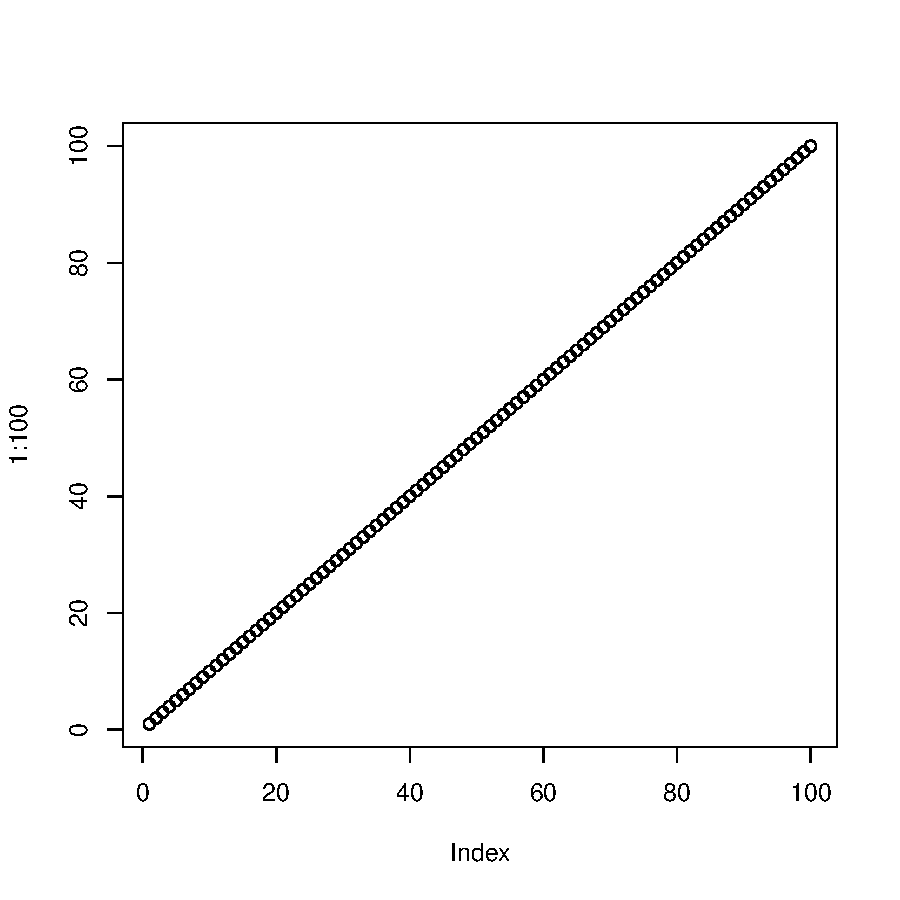
\includegraphics{Article-003}
\end{figure}
\bibliographystyle{natbib}
\bibliography{Article}
\end{document}
